\documentclass[11pt,letterpaper]{article}
\usepackage[T1]{fontenc}
\usepackage{lmodern,amsmath,amssymb,graphicx,xcolor,booktabs}
\usepackage[margin=.91in,top=.82in,bottom=.86in,headheight=15pt,headsep=15pt,footskip=29pt]{geometry}
\usepackage{fancyhdr}
\usepackage[colorlinks=true,allcolors=teal!65!black]{hyperref}
\hypersetup{pdftitle={A convex cover for every unit space curve},pdfauthor={OpenAI}}
\definecolor{ink}{HTML}{18374A}
\definecolor{accent}{HTML}{116E70}
\definecolor{pale}{HTML}{E9F3F1}
\setlength{\parindent}{0pt}
\setlength{\parskip}{5.5pt plus 1pt minus 1pt}
\setlength{\abovedisplayskip}{7pt plus 2pt}
\setlength{\belowdisplayskip}{7pt plus 2pt}
\pagestyle{fancy}\fancyhf{}
\fancyhead[L]{\small\sffamily\color{ink} Convex covers of unit space curves}
\fancyfoot[R]{\small\sffamily\color{ink}\thepage}
\renewcommand{\headrulewidth}{0.3pt}
\newcommand{\heading}[1]{{\large\sffamily\bfseries\color{ink}#1}\par\smallskip}
\newcommand{\term}[1]{\textbf{\color{ink}#1}}
\newcommand{\R}{\mathbb R}
\DeclareMathOperator{\area}{area}
\DeclareMathOperator{\vol}{vol}
\DeclareMathOperator{\TV}{TV}
\newcommand{\done}{\hfill\(\square\)}
\raggedbottom
\begin{document}
\thispagestyle{plain}
{\small\sffamily\color{accent} CONVEX GEOMETRY\hfill 19 NOVEMBER 2026\par}
\vspace{9pt}
{\fontsize{26}{30}\selectfont\sffamily\bfseries\color{ink} A convex cover for every\par unit space curve\par}
\vspace{7pt}
A smallest-volume convex body exists. Its exact volume and shape appear to be open. Let \(V_3\) denote that minimum. The bounds derived here are
\begin{center}
\setlength{\fboxsep}{10pt}\colorbox{pale}{\makebox[.83\linewidth]{\large
\(\displaystyle 0.0187328 < V_3 < 0.0542671.\)}}
\end{center}
The upper endpoint comes from an explicit body. Its middle slice is a planar quadrilateral that covers every unit plane curve. Above and below that slice the quadrilaterals shrink, with a flat cap at either end. The lower endpoint follows by considering three curves that every admissible body must fit, each in its own position and orientation.

\begin{center}
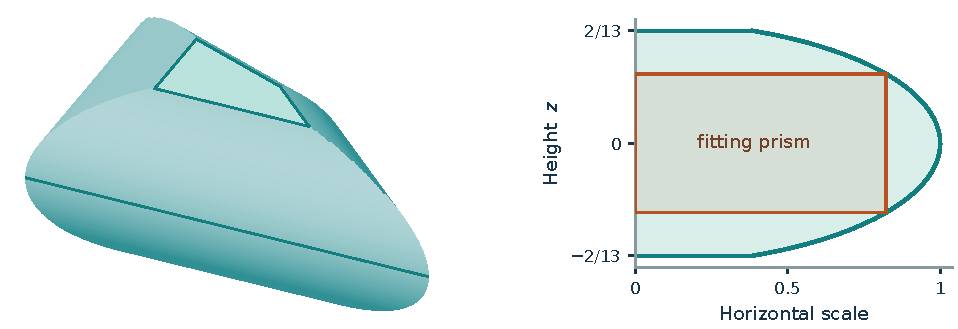
\includegraphics[width=.97\linewidth]{cover_figure.pdf}
\end{center}
{\small\sffamily\color{ink} The constructed body (left) and the scale of its horizontal slices (right). The rectangle shows how a prism enclosing a curve of vertical span \(0.19\) fits inside the body.\par}

\medskip
\term{Which curves and motions?} A curve is a continuous rectifiable path \(\gamma\colon[0,1]\to\R^3\) of arc length one. The body must contain its entire image. Endpoints are free and may coincide. A rigid placement has the form \(x\mapsto Rx+t\), with \(R\in SO(3)\). The body is compact and convex, and its boundary may be used. A shorter path can be extended to length one, so it is covered as well.

\term{Status of the estimates.} H\aa stad, Linusson and W\"astlund gave a three-dimensional cover of volume below \(0.075803\) \cite{HLW}. The bounds in the box use two 2026 preprints for a planar cover and a spatial width example \cite{Keller,Bartels}. Using the refereed planar sector theorem \cite{sector} and explicit elementary test curves gives the independent interval
\[
\frac{\sqrt3}{96}\ \le V_3\ \le\ \frac{121\pi}{6591}
\qquad (0.01804219\ldots\ \text{ to }\ 0.05767451\ldots).
\]

\newpage
\fontsize{12}{15.6}\selectfont
\heading{1. From a planar cover to a spatial one}
Let \(C\subset\R^2\) be a compact convex cover of every unit plane curve, translated so that \(0\in C\). Write \(A=\area(C)\), \(H=4/13\), and define
\begin{equation}
K_C=\left\{(x,z)\in\R^2\times\R:\ |z|\le H/2,\quad
 x\in\sqrt{1-36z^2}\,C\right\}.
\tag{1}
\end{equation}
\term{Covering theorem.} Every unit space curve fits in \(K_C\) by rotation and translation. Its volume is \((484/2197)A\).

The scale \(s(z)=\sqrt{1-36z^2}\) is concave on the defining interval. For \(0\le\lambda\le1\), convexity of \(C\) gives
\(\lambda s_1 C+(1-\lambda)s_2 C=(\lambda s_1+(1-\lambda)s_2)C\).
The copies \(sC\) are nested for \(s\ge0\) because \(0\in C\). These two facts give convexity of (1). Writing \(f(d)=\sqrt{1-9d^2}\), we see that the body contains the entire prism
\begin{equation}
f(d)C\,\times [-d/2,d/2]\qquad (0\le d\le H).
\tag{2}
\end{equation}
It suffices to find an orientation in which the curve has vertical span \(d\le H\) and its horizontal projection fits \(f(d)C\). A planar reflection used in fitting a projection extends to a proper spatial rotation by reversing the vertical coordinate too. The centered vertical interval in (2) accommodates this reversal.

\term{Alternating support planes.} For a space curve of full affine dimension, the generalized Wienholtz theorem gives two parallel supporting planes and four successive contacts, alternating between the planes \cite[Corollary 3.2]{Ghomi}. Take their normal as the vertical axis and write \(h\) for their separation. The vertical coordinate changes by \(h\) between each pair of successive contacts, so its total variation is at least \(3h\). For a curve lying in a plane, choose that plane as horizontal and set \(h=0\).

Parametrize by arc length and let \(p\) be the length of the horizontal projection. Applying the triangle inequality for integrals to the vector of horizontal and absolute vertical speeds gives
\[
\sqrt{p^2+\TV(z)^2}
=\left\|\int_0^1 (\|\gamma'_{\rm hor}(t)\|,|z'(t)|)\,dt\right\|
\le\int_0^1\|\gamma'(t)\|\,dt=1.
\]
Consequently \(h\le1/3\) and \(p\le s:=\sqrt{1-9h^2}\). If \(h\le H\), the projection fits \(sC\), and (2) covers the curve. Here a planar arc of length at most \(s\) fits \(sC\) by extension and scaling. The case \(s=0\) is interpreted as a point.

The remaining curves have \(H<h\le1/3\). In their current orientation they are too tall for (1), but their horizontal projections are short. Turning them on their sides gives the required placement.

\newpage
\heading{2. Why the ends can be cut off}
Suppose \(4/13\le h\le1/3\). In the horizontal plane choose a direction perpendicular to the projected endpoint displacement. If the displacement vanishes, choose any direction. In that coordinate the path begins and ends at the same value, so visiting both extremes and returning to the starting value costs at least twice its span \(q\) in total variation. Let \(a\) be the span in the other horizontal coordinate. Applying the speed inequality on the preceding page in two dimensions gives
\[
 a^2+4q^2\le p^2\le s^2=1-9h^2.
\]
Use the direction of span \(q\) as the new vertical. We have \(s\le5/13\), so \(q\le5/26<H\). The new horizontal footprint lies in an \(a\)-by-\(h\) rectangle. Walking along three of its sides, of lengths \(h,a,h\), gives a planar path whose convex hull is the rectangle. Thus the rectangle fits \((a+2h)C\).

To apply (2) it remains to check \(a+2h\le f(q)\). Since \(a\le s\le5h/4\), we have \(5(s+a)\le16h\), and hence
\[
9q^2\le\tfrac94(s-a)(s+a)
   \le(s-a)(s+a+4h)
   =(s+2h)^2-(a+2h)^2.
\]
Also \(s+2h\le1\), since \((1-2h)^2-s^2=h(13h-4)\ge0\) and \(1-2h\ge0\). These inequalities give \((a+2h)^2+9q^2\le1\), as required. Integrating the areas of the horizontal sections gives
\[
 \vol(K_C)=A\int_{-H/2}^{H/2}(1-36z^2)\,dz
      = A(H-3H^3)=\frac{484}{2197}A.\tag{3}
\]

\term{Two choices of base.} The circular sector of radius one and angle \(30^\circ\) is a planar cover by Panraksa and Wichiramala \cite{sector}. Its area \(\pi/12\) gives the upper bound \(121\pi/6591\). For the smaller construction use Keller's quadrilateral \cite[Theorem 4.1]{Keller}. To specify it exactly, put \(n(t)=(1-t^2,2t)/(1+t^2)\). Take the intersection of the half-planes \(n(t_i)\cdot x\le d_i\) with the parameters
\[
\begin{array}{c|rrrr}
 i&0&1&2&3\\ \hline
 t_i&-631/58&-1&7/16&37/56\\
 d_i&0&0&130783/250000&446199/1000000
\end{array}
\]
For the illustration, translate its vertex average to the origin. Intersecting consecutive lines and applying the shoelace formula gives the area on the left below. Equation (3) gives the corresponding spatial volume.
\[
A=\frac{7170601298323360123534337}{29109471743520000000000000},
\qquad
\vol(K_C)=0.05426709276528461389\ldots.
\]

\newpage
\heading{3. Three curves force a positive volume}
The \emph{minimum width} of a subset of a Euclidean space is the smallest distance between parallel supporting hyperplanes in that space. Consider a planar unit curve of planar minimum width \(b\), and a spatial unit curve of spatial minimum width \(w\). Together with a straight unit segment, these curves force
\begin{equation}
                   V_3\ \ge\ \frac{bw}{6}.
\tag{4}
\end{equation}

\term{The shadow.} Let \(K\) be any admissible body. Choose a unit segment in \(K\) of direction \(u\), and project \(K\) orthogonally onto \(u^\perp\), obtaining a planar convex set \(P\). The plane of the placed planar curve contains a direction parallel to \(u^\perp\). Width in that direction survives projection, giving \(\operatorname{diam}(P)\ge b\). Every direction in \(u^\perp\) is also a direction of the placed spatial curve, giving \(\operatorname{width}(P)\ge w\).

Take a diameter of \(P\) as a base segment, and a point of greatest signed distance on each side of its line. The two triangles they span with the base have disjoint interiors, and their heights add to the width normal to the line. They lie in \(P\). Thus \(\area(P)\ge bw/2\).

\term{The fibers.} For \(y\in P\), write \(\ell(y)\) for the length of the interval \(K\cap(y+\R u)\). At the projected unit segment \(y_0\) this length is at least one. Combining a point of the fiber over \(y\) with both segment endpoints gives, by convexity, \(\ell((1-t)y+ty_0)\ge t\) for \(0\le t\le1\). Thus \(\{\ell\ge t\}\) contains a copy of \(P\) scaled by \(1-t\). Integration yields
\[
 \vol(K)=\int_P\ell(y)\,dy\ \ge\ \area(P)\int_0^1(1-t)^2\,dt
       =\frac{\area(P)}{3}\ \ge\ \frac{bw}{6}.\qquad\square
\]

\term{The numerical lower bound.} Adhikari and Pitman's planar caliper has width one and length less than \(2.27830\) \cite{caliper}. Bartels, Choy, Wu and Li give a space curve of width one and length less than \(3.905124162243594\) \cite[Theorem 1]{Bartels}. Rescaling each to length one and applying (4) gives
\[
 V_3>\frac{1}{6\cdot2.27830\cdot3.905124162243594}
      =0.0187328127825304\ldots .
\]
Only the existence of those individual curves is needed. The question of which spatial curve has greatest width at length one is a separate optimization problem.

\term{An elementary choice.} For the planar curve take two consecutive sides of an equilateral triangle of side \(1/2\). The minimum width of its hull is its altitude \(b=\sqrt3/4\) (the minimum width of a triangle is normal to one of its edges). The four-link curve on the next page gives \(w=1/4\). These two examples prove \(V_3\ge\sqrt3/96\) without either width estimate from the literature.

\newpage
\heading{4. A four-link curve of width one quarter}
Consider the polygonal path through these five successive vertices.
\[
 (\sqrt{15},0,0),\quad(0,-3,4),\quad(0,0,5),\quad(0,3,4),\quad(-\sqrt{15},0,0).
\]
Together the two outer links of length \(2\sqrt{10}\) and the two inner links of length \(\sqrt{10}\) have length \(6\sqrt{10}\). Write \(W(v)\) for the difference of the largest and smallest dot products of the five vertices with a vector \(v\). Extremes on a straight link occur at its ends, so this is also the directional spread of the path. By homogeneity its minimum width is the reciprocal of the largest \(\|v\|\) for which \(W(v)\le1\).

Reflections in the coordinate planes \(x=0\) and \(y=0\) preserve the vertex set, and negating the whole vector preserves its spread. We may therefore assume \(v=(x,y,z)\) has nonnegative coordinates. Set \(a=\sqrt{15}\,x,\ b=3y,\ c=z\). Then
\[
 W(v)=\max(a,b+4c,5c)+\max(a,b-4c).
\]
Expanding the maxima shows that \(W(v)\le1\) is equivalent to
\[
 0\le a,b\le\tfrac12,\qquad c\ge0,\qquad
 a+b+4c\le1,\qquad a+5c\le1 .
\]
Indeed the other pairwise sums give redundant inequalities, including \(b+c\le1\), which follows from \(b\le1/2\) and \(c\le1/5\).

The convex quadratic \(Q=\|v\|^2=a^2/15+b^2/9+c^2\) attains a maximum at a vertex of this bounded polytope. Intersecting triples of its seven boundary planes and retaining feasible points gives the following complete list.
\begin{center}\small
\begin{tabular}{cccc@{\hspace{.7in}}cccc}
\toprule
\(a\)&\(b\)&\(c\)&\(Q\)&\(a\)&\(b\)&\(c\)&\(Q\)\\
\midrule
0&0&0&0&$1/2$&0&0&$1/60$\\
0&0&$1/5$&$1/25$&$1/2$&0&$1/10$&$2/75$\\
0&$1/5$&$1/5$&$2/45$&$1/2$&$1/10$&$1/10$&$1/36$\\
0&$1/2$&0&$1/36$&$1/2$&$1/2$&0&$2/45$\\
0&$1/2$&$1/8$&$25/576$&&&&\\
\bottomrule
\end{tabular}
\end{center}
Thus \(\max Q=2/45\). The unscaled minimum width is \(\sqrt{45/2}\). Dividing by the length \(6\sqrt{10}\) gives the claimed unit-length width of \(1/4\). \done

\term{Reproducing the calculations.} Run \texttt{python3 check\_width.py} to reproduce the vertex table, and \texttt{python3 check\_bounds.py} for the base area and volume. Both scripts use rational arithmetic for the finite checks. The geometric covering properties of the planar bases and the two literature width estimates enter as cited theorems.

\newpage
\heading{5. Why a minimizing body exists}
A uniform volume bound by itself need not bound the diameters of convex bodies. For this problem a single forced curve supplies the missing control.

Take a regular tetrahedron of edge \(1/3\). Visiting its four vertices along three edges gives a unit curve. Each admissible body contains its placed convex hull, hence a ball of fixed radius \(r=\sqrt6/36\), the inradius of the tetrahedron. Translate this ball's center to the origin. If \(x\ne0\) lies in the body, the disk of radius \(r\) in \(x^\perp\) centered at the origin also lies in it. The cone from the disk to \(x\) lies in the body by convexity, so
\[
 \|x\|\le\frac{3\vol(K)}{\pi r^2}.
\]

Now take a minimizing sequence. Its volumes are bounded, so all the translated bodies lie in one fixed ball. The Blaschke selection theorem gives a subsequence converging in the Hausdorff metric to a compact convex set \(K_\ast\). It contains the fixed ball of radius \(r\). Volume is continuous for Hausdorff convergence of compact convex bodies, so its volume is the proposed infimum.

For each fixed curve, put its initial point at the origin and consider its placements in this subsequence. The rotations belong to the compact group \(SO(3)\), and the translations lie in the common bounding ball. Extract a convergent subsequence of placements. Its limit places the curve in \(K_\ast\) by Hausdorff convergence. The subsequence can depend on the curve because the limiting body is already fixed. Thus \(K_\ast\) is universal and attains \(V_3\). \done

\term{Further questions.} How much more can the ends of (1) be trimmed if one uses the actual side directions of Keller's quadrilateral? Can a lower bound exploit the full convex hulls of the three test curves, beyond the two widths in (4)?

\vspace{4pt}
\begingroup\small
\renewcommand{\refname}{Sources}
\begin{thebibliography}{9}\setlength{\itemsep}{3pt}\setlength{\parskip}{0pt}
\bibitem{HLW} J. H\aa stad, S. Linusson and J. W\"astlund. A smaller sleeping bag for a baby snake. \emph{Discrete Comput. Geom.} 26 (2001), 173--181.
\href{https://doi.org/10.1007/s00454-001-0011-5}{doi:10.1007/s00454-001-0011-5}.
\bibitem{Ghomi} M. Ghomi. The length, width, and inradius of space curves. \emph{Geom. Dedicata} 196 (2018), 123--143. \href{https://ghomi.math.gatech.edu/Papers/inradius.pdf}{Author's paper}, Corollary 3.2.
\bibitem{sector} C. Panraksa and W. Wichiramala. Wetzel's sector covers unit arcs. \emph{Period. Math. Hungar.} 82 (2021), 213--222. \href{https://doi.org/10.1007/s10998-020-00354-x}{doi:10.1007/s10998-020-00354-x}.
\bibitem{Keller} E. Keller. Improved bounds for universal convex covers of unit arcs. Preprint, 2026. \href{https://arxiv.org/abs/2609.21968}{arXiv:2609.21968}, Theorem 4.1.
\bibitem{caliper} A. Adhikari and J. Pitman. The shortest planar arc of width 1.
\emph{Amer. Math. Monthly} 96 (1989), 309--327. \href{https://doi.org/10.1080/00029890.1989.11972188}{doi:10.1080/00029890.1989.11972188}.
\bibitem{Bartels} T. S. Bartels, D. K. Choy, R. Wu and T. Li. A short open space curve of unit width. Preprint, 2026. \href{https://arxiv.org/abs/2610.19585}{arXiv:2610.19585}, Theorem 1.
\end{thebibliography}
\endgroup
\end{document}
